\documentclass{beamer}

\usepackage[utf8]{inputenc}


%Information to be included in the title page:
\title{\centering
\includegraphics[width=\textwidth]{../img/title.pdf}}
\author{Tyler Chen}
\institute{}
\date{May 30, 2018}

\setbeamertemplate{bibliography item}{\insertbiblabel}
\input{../../../import/mathsymbols.tex} % Math shortcuts
\usepackage{subcaption}

\usefonttheme{professionalfonts}
\newcommand{\indep}{\rotatebox[origin=c]{90}{$\models$}}
\usepackage{fontspec}

\renewcommand{\d}{\ensuremath{\mathrm{d}}}

\begin{document}

\frame{\setsansfont{Comic Sans MS}\titlepage}

\begin{frame}
\frametitle{Why do we want to study SDEs?}
\begin{itemize}
    \item Model physical systems (molecular dynamics, neurodynamics)
    \item Make \$\$\$\$ (sell soul and model financial things)
    \item solve PDEs (avoid efficiency issues in high dimensions)
\end{itemize}
\end{frame}

\begin{frame}
\frametitle{Brownian Motion}
Brownian motion is characterized by four properties,
\begin{enumerate}
    \item \( W_0 = 0 \)
    \item \( (W_d-W_c) \indep (W_b-W_a) \) for \( 0\leq a\leq b\leq c\leq d \))
    \item \( (W_t - W_s) \sim \mN(0,t-s) \) for \( 0\leq s\leq t \)
    \item the map \( t \to W_t \) is continuous almost surely
\end{enumerate}
\end{frame}

\begin{frame}
\frametitle{What is an SDE?}
\begin{itemize}
    \item A Stochastic Differential Equation (SDE) is an equation of the form,
    \begin{align*}
    \d X_t =  \mu(X_t,t)\d t + \sigma(X_t,t)\d W_t
    \end{align*}
    where \( W_t \) denotes a standard Brownian Motion \cite{lorig}.
    \item This has solution,
    \begin{align*}
    X_{T} - X_{0} = \int_{0}^{T} \mu(t,X_t)\d t + \int_{0}^{T} \sigma(t,X_t) \d W_t
    \end{align*}
\end{itemize}

\end{frame}


\begin{frame}
\frametitle{A Simple Numerical Method}

\begin{itemize}
\item Approximating each integral in the simplest way gives,
\begin{align*}
    \hat{X}_{t+\Delta t} &= \hat{X}_t + \mu(t,\hat{X}_{t}) \Delta t + \sigma(t,\hat{X}_{t}) \Delta W_{t}
\end{align*}

\item Given timestep \( \Delta t \) we sample \( \Delta W_t \), where \( \Delta W_t \sim  \mN(0,\Delta t) \).
\item This method is referred to as the Euler-Maruyama Method \cite{sdes}.
\end{itemize}

\end{frame}

\begin{frame}
\frametitle{Convergence}
\begin{itemize}
\item Strong Convergence tells us individual trajectories converge
\begin{align*}
    \lim_{\Delta t\to 0}\bE\left[\left| X_T - \hat{X}_T \right|\right] = 0
\end{align*}

\item Weak Convergence tells us the statistics (mean and higher moments) converge
\begin{align*}
    \lim_{k\to 0} \left| \bE\left[ p(X_T) - p(\hat{X}_T) \right] \right| = 0
\end{align*}
\end{itemize}
\end{frame}

\begin{frame}
\frametitle{Higher Order (Taylor) Methods}
\begin{itemize}
\item Higher order methods can be derived from stochastic Taylor expansion
\item Recall It\^o's Lemma
{\footnotesize
\begin{align*}
    f(T,X_T) &= f(t,X_t) + \int_t^T \mM f(s,X_s)\d s + \int_t^T \mS f(s,X_s) \d W_s \label{ito1}
\end{align*}}
{\footnotesize
\begin{align*}
    \mM := \pp{}{s} +  \mu(s,X_s)\pp{}{x} + \frac{1}{2}\sigma^2(s,X_s) \pp[2]{}{x}, && \mS := \sigma(s,X_s) \pp{}{x}
\end{align*}}
\end{itemize}
\end{frame}

\begin{frame}
\frametitle{Euler-Maruyama Method}
\begin{itemize}
\item Apply previous identity to \( \mu \) and \( \sigma \) to obtain,
{\scriptsize
\begin{align*}
    X_{T} - X_{0} &= \int_{0}^{T} \mu(t,X_t)\d t + \int_{0}^{T} \sigma(t,X_t) \d W_t \\
    &= X_t + \mu(t,X_t) \int_t^T \d s +  \sigma(t,X_t)\int_t^T \d W_s + R
\end{align*}}
where,
{\scriptsize
\begin{align}
    R &=  \int_t^T \int_t^s \mM \mu(u,X_u) \d u \d s + \int_t^T \int_t^s \mS \mu(u,X_u)\d W_u  \d s \tag*{}
    \\ &\hspace{4em} + \int_t^T \int_t^s \mM \sigma(u,X_u)\d u \d W_s + \int_t^T \int_t^s \mS \sigma(u,X_u) \d W_u \d W_s
\end{align}}
\end{itemize}
\end{frame}

\begin{frame}
\frametitle{Milstein Method}
\begin{itemize}
\item using the heursitics the \( \d W_u \d W_s \) term is lowest order
\item use identity on \( \mS \sigma \) to obtain,
{
\begin{align*}
    X_T &= X_t + \int_t^T \mu(t,X_t) \d s + \int_t^T \sigma(t,X_t) \d W_s
    \\&\hspace{5em} + \int_t^T \int_t^s \mS \sigma(t,X_t)  \d W_u \d W_v + R
\end{align*}}
\item This gives the Millstein method,
\begin{align*}
    \hat{X}_{t+\Delta t} &= \hat{X}_t + \mu(t,\hat{X}_{t}) \Delta t + \sigma(t,\hat{X}_{t}) \Delta W_{t}
    \\& \hspace{4em}+ \sigma(t,\hat{X}_t) \partial_x \sigma(t,\hat{X}_t) \left( (\Delta W_t)^2 - \Delta t \right)/2
\end{align*}
\end{itemize}
\end{frame}

\begin{frame}
\frametitle{Runge Kutta Method}
\begin{itemize}
\item Expand integral form of solution using It\^o's lemma and drop terms of \( \mO(\d t) \)
\item Replace derivatives with finite difference
\begin{align*}
    \hat{X}_{t+\Delta t} &= \hat{X}_t + \mu(t,\hat{X}_{t}) \Delta t + \sigma(t,\hat{X}_{t}) \Delta W_{t}
    \\& \hspace{3em} + \sigma(t,\hat{X}_t-X^*) \left( (\Delta W_t)^2 - \Delta t \right) / (2 \sqrt{\Delta t}) \\
    X^* &=  \hat{X}_t  + \sigma(t,\hat{X}_t)\sqrt{\Delta t}
\end{align*}

\end{itemize}
\end{frame}


\begin{frame}
\frametitle{Tests of Weak Convergence}
OU process with \( \theta = 2, \mu=1,\sigma=1/100, T=1 \), 5000 trajectories
\begin{figure}[ht!]\centering
\begin{subfigure}{.48\textwidth}\centering
    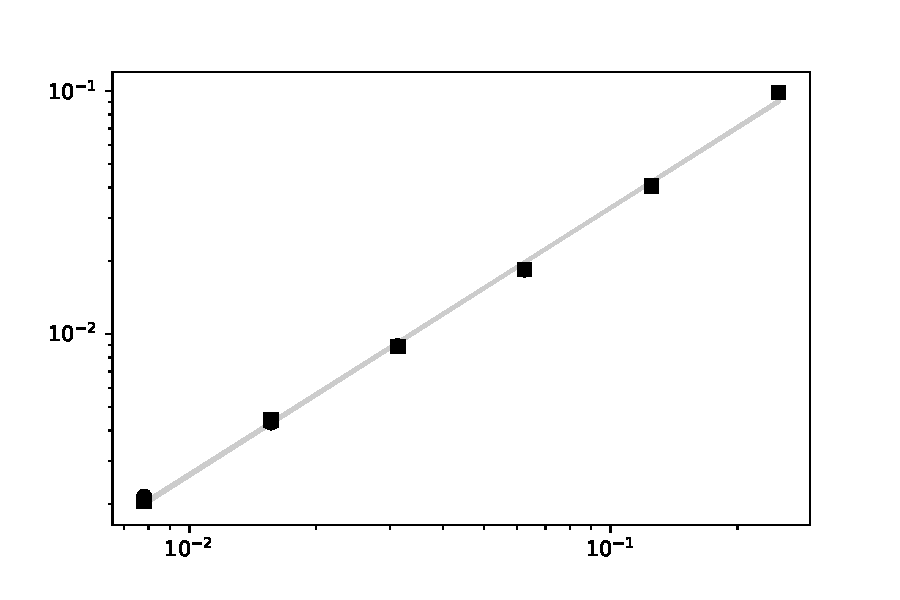
\includegraphics[width=\textwidth]{../img/weak_order_5000.pdf}
    \caption{\tiny\( \big|\bE[X_T] - \bE[\hat{X}_T]\big| \)}
    \label{mean}
\end{subfigure}
\begin{subfigure}{.48\textwidth}\centering
    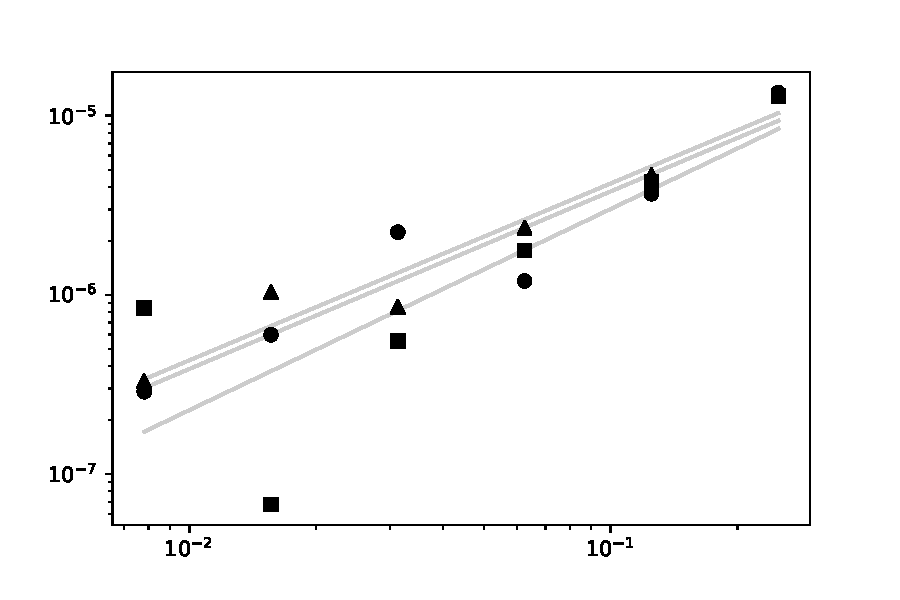
\includegraphics[width=\textwidth]{../img/weak_order_var_5000.pdf}
    \caption{\tiny\( \big|\bE[(X_T-\bE[X_T])^2] - \bE[(\hat{X}_T-\bE[X_T])^2]\big| \) }
    \label{var}
\end{subfigure}
\caption{Circles: Euler--Maruyama, triangles:  Runge-Kutta, squares: Euler--Maruyama with \( \Delta W_t \in \{-\Delta t, \Delta t\} \). }
\label{weak_order_test}
\end{figure}
Note that all slopes are about 1
\end{frame}

\begin{frame}
\frametitle{Tests of Strong Convergence}
 Geometric Brownian motion with \( \mu = 1, \sigma = 1/2, T=8 \), 300 trajectories

\begin{figure}[ht!]\centering
    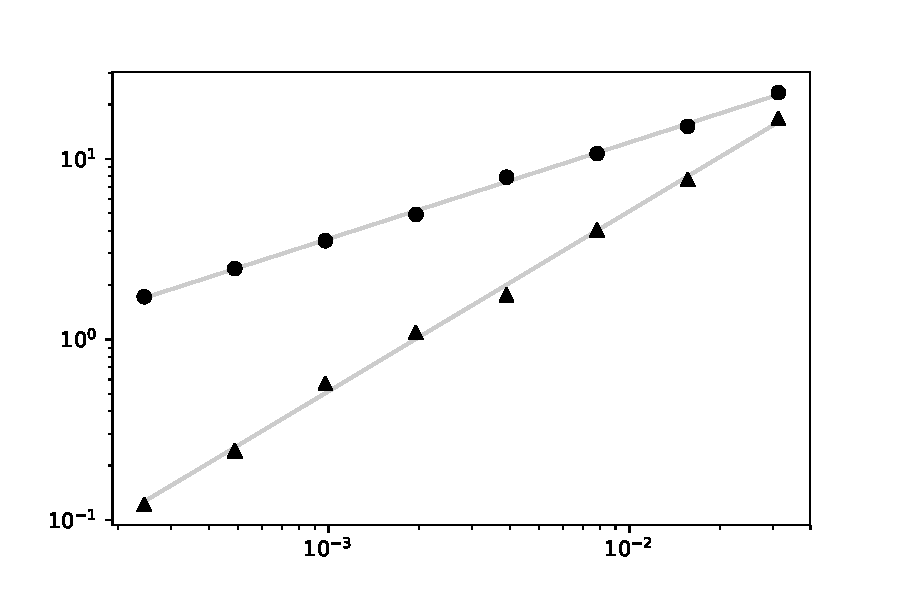
\includegraphics[width=.5\textwidth]{../img/strong_order_300.pdf}
    \caption{Values of \( \bE|X_T - \hat{X}_T| \), circles: Euler--Maruyama, triangles: Runge-Kutta}
\label{strong_order_test}
\end{figure}

Note that all slopes are about 1/2 and 1 for EM and RK respectively.
\end{frame}

\begin{frame}
\frametitle{References}
    \bibliography{../project}{}
    \bibliographystyle{amsplain}
\end{frame}
\end{document}
